
\documentclass{beamer}

\usepackage{graphicx}
\usepackage[latin1]{inputenc}
\usepackage[T1]{fontenc}
\usepackage[english]{babel}
\usepackage{listings}
\usepackage{xcolor}
\usepackage{eso-pic}
\usepackage{mathrsfs}
\usepackage{url}
\usepackage{amssymb}
\usepackage{amsmath}
\usepackage{multirow}
\usepackage{hyperref}
\usepackage{booktabs}
% \usepackage{bbm}
\usepackage{cooltooltips}
\usepackage{colordef}
\usepackage{beamerdefs}
\usepackage{lvblisting}

\usepackage{multimedia}
\usepackage{algorithmicx}
\usepackage[noend]{algpseudocode}
\usepackage{algorithm}


\pgfdeclareimage[height=2cm]{logobig}{hulogo}
\pgfdeclareimage[height=0.7cm]{logosmall}{Figures/LOB_Logo}

\renewcommand{\titlescale}{1.0}
\renewcommand{\titlescale}{1.0}
\renewcommand{\leftcol}{0.6}


\title[Eigenvalue Problems - Numerical Solutions]{Eigenvalues and Eigenvectors}
\authora{Thomas Siskos}
\authorb{}
\authorc{}

\def\linka{siskosth@student.hu-berlin.de}
\def\linkb{http://github.com/thsis/NIS18}
\def\linkc{}

\institute{Numerical Introductory Seminar \\
Humboldt--University Berlin \\}

\hypersetup{pdfpagemode=FullScreen}

\begin{document}
% 0-1
%%%%%%%%%%%%%%%%%%%%%%%%%%%%%%%%%%%%%%%%
\frame[plain]{

\titlepage
}

\frame{
  \frametitle{Agenda}
  \tableofcontents
}
%%%%%%%%%%%%%%%%%%%%%%%%%%%%%%%%%%%%%%%%

\section{Motivation}
\frame[containsverbatim]{
\frametitle{PCA}
\begin{columns}[onlytextwidth]
\begin{column}{0.25\textwidth}
	\begin{itemize}
		\item The iris dataset is already linearly separable.
		\item With various techniques we can show this in even more detail.
	\end{itemize}
\end{column}
\begin{column}{0.75\textwidth}
\begin{figure}
  	\begin{center}
	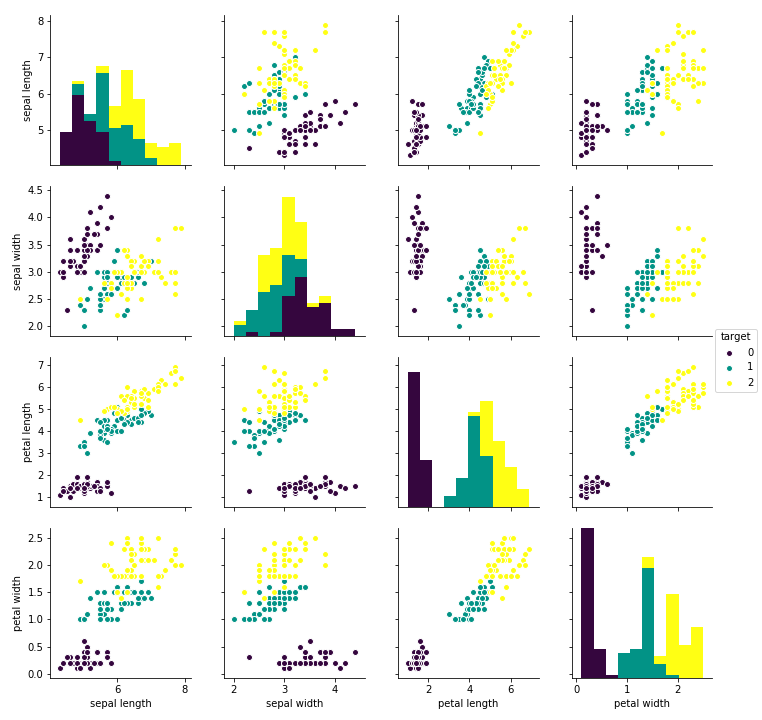
\includegraphics[scale=0.20]{../media/plots/iris_raw.png}
    \caption{\href {https://github.com/thsis/NIS18/blob/master/tests/tests_models.py}{Iris Pairplot}  \protect\includegraphics[scale=0.05]{qletlogo.pdf}}
	\end{center}
\end{figure}
\end{column}
\end{columns}
}

%%%%%%%%%%%%%%%%%%%%%%%%%%%%%%%%%%%%%%%%%%%%%%%%%%%%%%%%%%%%%%%%%%%%%%%%%%%%%%%%%%%%%%%%%%%%%%%%%%%%%%%%

\frame[containsverbatim, label=PCA-prop]{
\frametitle{PCA}
\begin{columns}[onlytextwidth]
\begin{column}{0.65\textwidth}
	\begin{itemize}
		\item objective:
		\begin{equation}
		\label{pca_obj}
            max\ \delta^{\prime} Var \left(X\right) \delta \; s.t. \; \sum \delta_i^2 = 1.
        \end{equation}
        where $X \in \mathbb{R}^{n \times m}; m,n \in \mathbb{N}; \delta \in \mathbb{R}^m$
		\item solution \hyperlink{PCA-proof}{\beamergotobutton{Proof}}
:
		\begin{equation}
		\label{pca_sol}
			Y = \Gamma^{\prime} \left(X - \mu\right)
		\end{equation}
		where $Y \in \mathbb{R}^{n \times m}$ is the matrix of rotations,
		      $\Gamma \in \mathbb{R}^{m \times m}$ is the matrix of eigenvectors,
		      $\mu \in \mathbb{R}^m$ is the vector of sample means.
	\end{itemize}
\end{column}
\begin{column}{0.35\textwidth}
\begin{figure}
	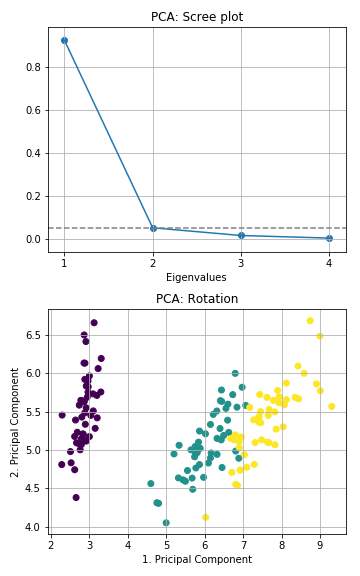
\includegraphics[width=3.5cm, height=5cm]{../media/plots/iris_pca.png}
	\caption{\href {https://github.com/thsis/NIS18/blob/master/tests/tests_models.py}{Iris PCA}  \protect\includegraphics[scale=0.05]{qletlogo.pdf}}
\end{figure}
\end{column}
\end{columns}
}

%%%%%%%%%%%%%%%%%%%%%%%%%%%%%%%%%%%%%%%%%%%%%%%%%%%%%%%%%%%%%%%%%%%%%%%%%%%%%%%%%%%%%%%%%%%%%%%%%%%%%%%%

\frame{
\frametitle{LDA}
\begin{itemize}
	\item objective:
		\begin{equation}
		\label{lda_obj}
  			max \ \frac{w^{\prime}S_B w}{w^{\prime}S_W w},
		\end{equation}
	where
	\begin{align*}
  	S_B &= \sum\limits_{c}^{C} (\mu_c - \mu)(\mu_c - \mu)^{\prime}, \\
  	S_W &= \sum\limits_{c}^{C} \sum\limits^{n}_{i=1} (x_i - \mu_c)(x_i - \mu_c)^{\prime}
	\end{align*}
	and $x_i \in \mathbb{R}^m$, $\mu_c$ is the vector of class means.
\end{itemize}

}

%%%%%%%%%%%%%%%%%%%%%%%%%%%%%%%%%%%%%%%%%%%%%%%%%%%%%%%%%%%%%%%%%%%%%%%%%%%%%%%%%%%%%%%%%%%%%%%%%%%%%%%%

\frame[containsverbatim, label=LDA-prop]{
\frametitle{LDA}
\begin{columns}[onlytextwidth]
\begin{column}{0.65\textwidth}
\begin{itemize}
\item solution \hyperlink{LDA-proof}{\beamergotobutton{Proof}}:
\begin{equation}
  \label{lda_sol}
    S_B^{\frac{1}{2}}S_{W}^{-1}S_B^{\frac{1}{2}} v = \lambda v
  \end{equation}
  with $$    v = S_B^{\frac{1}{2}} w, $$ where this is again an Eigenvalue problem and it's solution will provide the rotation that ensures the largest possible (linear) separability.
\item Now how do we get the Eigenvalues?
\end{itemize}
\end{column}
\begin{column}{0.35\textwidth}
\begin{figure}
	\begin{center}
	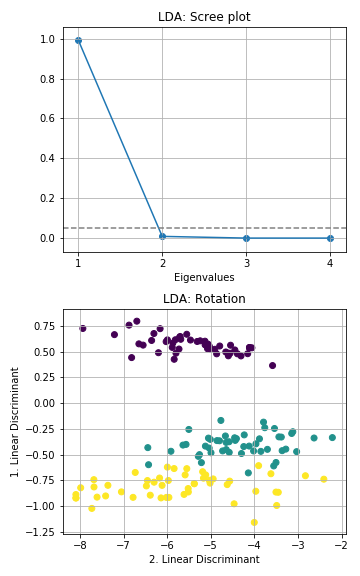
\includegraphics[width=3.5cm, height=5cm]{../media/plots/iris_lda.png}
	\caption{\href {https://github.com/thsis/NIS18/blob/master/tests/tests_models.py}{Iris LDA}  \protect\includegraphics[scale=0.05]{qletlogo.pdf}}
	\end{center}
\end{figure}
\end{column}
\end{columns}
}

%%%%%%%%%%%%%%%%%%%%%%%%%%%%%%%%%%%%%%%%%%%%%%%%%%%%%%%%%%%%%%%%%%%%%%%%%%%%%%%%%%%%%%%%%%%%%%%%%%%%%%%%

\section{Key Idea \& Definitions}
\frame{
\frametitle{Eigenvalue}
If $A$ is an $n \times n$ matrix, $v$ is a non-zero vector and $\lambda$ is a scalar, such that
\begin{equation}
\label{eigenvalue-def}
Av = \lambda v
\end{equation}
then $v$ is called an \textit{eigenvector} and $\lambda$ is called an \textit{eigenvalue} of the matrix $A$.
An eigenvalue of A is a root of the characteristic equation,
\begin{equation}
\label{eigenvalue-solve}
det\left(A - \lambda I \right) = 0
\end{equation}
}

%%%%%%%%%%%%%%%%%%%%%%%%%%%%%%%%%%%%%%%%%%%%%%%%%%%%%%%%%%%%%%%%%%%%%%%%%%%%%%%%%%%%%%%%%%%%%%%%%%%%%%%%

\subsection{Characteristic Polynomial \& Diagonal Matrices}
\frame[label=companion_prop]{
\frametitle{The characteristic polynomial}
Consider the polynomial
\begin{equation}
\label{characteristic-polynomial}
f(\lambda) = \lambda^p + a_{p-1}\lambda^{p-1} + \dots + a_1 \lambda + a_0
\end{equation}
We now construct a matrix $A \in \mathbb{R}^{n \times n}$ such that the eigenvalues of $A$ are the roots of the polynomial $f(\lambda)$ \hyperlink{companion_exmpl}{\beamergotobutton{Example}}:
\begin{equation}
\label{companion-matrix}
A = \begin{bmatrix}
        0    & 1    & 0    & \dots & 0 \\
        0    & 0    & 1    & \cdots & 0 \\
             &      &      & \ddots & \\
        0    & 0    & 0    & \dots  & 1 \\
        -a_0 & -a_1 & -a_2 & \dots  & -a_{p-1} \\
    \end{bmatrix}
\end{equation}
}

%%%%%%%%%%%%%%%%%%%%%%%%%%%%%%%%%%%%%%%%%%%%%%%%%%%%%%%%%%%%%%%%%%%%%%%%%%%%%%%%%%%%%%%%%%%%%%%%%%%%%%%%

\subsection{Similarity Transformations}
\frame[containsverbatim]{
\frametitle{General Idea}

What are the eigenvalues of $X_1$ and $X_2$?

\begin{columns}[onlytextwidth]
\begin{column}{0.3\textwidth}
\begin{equation*}
X_1 = \begin{bmatrix}
1 & 0 & 0 & 0 \\
0 & 2 & 0 & 0 \\
0 & 0 & 3 & 0 \\
0 & 0 & 0 & 4 \\
\end{bmatrix}
\end{equation*}
\end{column}
\begin{column}{0.7\textwidth}
\begin{equation*}
X_2 = \begin{bmatrix}
        2.297 & -0.461 & -0.459 &  0.225 \\
       -0.461 &  1.4   & -0.097 & -0.829 \\
       -0.459 & -0.097 &  2.672 &  0.224 \\
        0.225 & -0.829 &  0.224 &  3.631 \\
\end{bmatrix}
\end{equation*}
\end{column}

\end{columns}
}

\frame[label=similarity_prop]{
\frametitle{Similarity Transformations}

Two $n \times n$ matrices $A$ and $B$, are said to be \textit{similar} if there exists a nonsingular matrix $P$ such that
\begin{equation}
\label{similarity-prop}
A = P^{-1} B P
\end{equation}

If the two matrices $A$ and $B$ are similar, then they also share the same eigenvalues. \hyperlink{similarity_proof}{\beamergotobutton{Proof}}
}

%%%%%%%%%%%%%%%%%%%%%%%%%%%%%%%%%%%%%%%%%%%%%%%%%%%%%%%%%%%%%%%%%%%%%%%%%%%%%%%%%%%%%%%%%%%%%%%%%%%%%%%%

\subsubsection{Householder Reflections}
\frame[label=householder_prop]{
\frametitle{Householder Reflections}
Let $u$ and $v$ be orthonormal vectors and let $x$ be a vector in the space spanned by $u$ and $v$, such that
$$x = c_1 u + c_2 + v$$
for some scalars $c_1$ and $c_2$. The vector
$$\tilde{x}=-c_1 u + c_2 v$$
is a \textit{reflection} of x through the line difined by the vector u. Now consider the matrix

\begin{equation}
Q = I - 2 uu^{\prime}.
\end{equation}

Note that \hyperlink{householder_proof}{\beamergotobutton{Proof}}:
$$Qx = \tilde{x}$$
}

\frame{
\frametitle{Householder Reflections}
We will use Householder-Reflections to tranform a vector
$$a = (a_1, \dots, a_n)$$
into
$$\hat{a} = (\hat{a}_1, 0, \dots, 0)$$
}
%%%%%%%%%%%%%%%%%%%%%%%%%%%%%%%%%%%%%%%%%%%%%%%%%%%%%%%%%%%%%%%%%%%%%%%%%%%%%%%%%%%%%%%%%%%%%%%%%%%%%%%%

\subsubsection{Givens Rotations}
\frame[containsverbatim]{
\frametitle{Givens Rotations}
Using orthogonal transformations we can also rotate a vector in such a way that a specified element becomes 0 and only one other element in the vector is changed.

\begin{columns}[onlytextwidth]
\begin{column}{0.5\textwidth}
$$
Q = \begin{bmatrix}
\cos\theta & \sin\theta \\
-\sin\theta & \cos\theta
\end{bmatrix}
$$
\end{column}
\begin{column}{0.5\textwidth}
	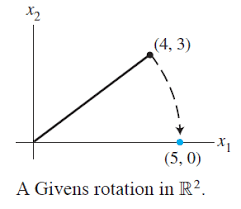
\includegraphics[scale=.5]{../media/plots/givens.png}
\end{column}
\end{columns}



}
\frame[label=givens_prop]{
\frametitle{Givens Rotations}

\begin{equation}
V_{pq}(\theta) = \begin{bmatrix}
                      1 &  &  &  &  &  &  &  &  \\
                       & \ddots &  &  &  &  & &  &  \\
                       &  & 1 &  &  &  &  &  &  \\
                       &  &  & \cos\theta &  & \sin\theta &  &  &  \\
                       &  &  &  & \ddots &  &  &  &  \\
                       &  &  & -\sin\theta &  & \cos\theta &  &  &  \\
                       &  &  &  &  &  & 1 &  &  \\
                       &  &  &  &  &  &  & \ddots &  \\
                       &  &  &  &  &  &  &  & 1 \\
                 \end{bmatrix}
\end{equation}
	where $\cos\theta = \frac{x_p}{||x||}$ and $\sin\theta = \frac{x_q}{||x||}$

}
%%%%%%%%%%%%%%%%%%%%%%%%%%%%%%%%%%%%%%%%%%%%%%%%%%%%%%%%%%%%%%%%%%%%%%%%%%%%%%%%%%%%%%%%%%%%%%%%%%%%%%%%

\section{Algorithms}
\subsection{Jacobi-Method}
\frame{
\frametitle{Jacobi Method}

The Jacobi method for determining the eigenvalues of a symmetric matrix $A$ uses a sequence of orthogonal similarity transformations that result in the transformation:
$$A = P  \Lambda P^{-1}$$ or rather: $$\Lambda=P^{-1}AP$$
where we use Givens Rotations to obtain $P$. The Jacobi iteration is:
\begin{equation}
\label{j-meth}
A^{k} = V_{p_k q_k}(\theta_k)A^{k-1}V_{p_k q_k}(\theta_k)
\end{equation}

The Jacobi Method is of $O(n^3)$
}
%%%%%%%%%%%%%%%%%%%%%%%%%%%%%%%%%%%%%%%%%%%%%%%%%%%%%%%%%%%%%%%%%%%%%%%%%%%%%%%%%%%%%%%%%%%%%%%%%%%%%%%%
\frame{
\frametitle{Jacobi-Method}
\begin{algorithm}[H]
\caption{\texttt{jacobi}}
\label{j-algo}
\begin{algorithmic}
  \Require symmetric matrix $A$
  \Ensure $0 < precision < 1$
  \Statex \textbf{initialize: } $L \gets A$; $U \gets I$; $L_{max} \gets 1$
  \While{$L_{max} > precision$}
    \State Find indices $i$, $j$ of largest value in lower triangle of $abs(L)$
        \State $L_{max} \gets L_{i,j}$
            \State $\alpha \gets \frac{1}{2}\cdot \arctan(\frac{2A_{i, j}}{A_{i, i}-A_{j, j}})$
    \State $V \gets I$
    \State $V_{i, i}, V_{j, j} \gets \cos \alpha$; $V_{i, j}, V_{j, i} \gets -\sin \alpha, \sin \alpha$
    \State $A \gets V^{\prime} A V$; $U \gets UV$

  \EndWhile
  \Return $diag(A), U$
\end{algorithmic}
\end{algorithm}
}
\subsection{QR-Method}
\frame{
\frametitle{QR-Method}
The QR-Method is the most common algorithm for obtaining eigenvalues and eigenvectors of a matrix $A$. It relies on the so called QR-Factorization:
\begin{equation}
A = QR,
\end{equation}
where $Q$ is an orthogonal and $R$ is an upper triangular matrix. \\
The QR iteration is:
\begin{equation}
  A^k = Q_{k-1}^{\prime} A_{k-1} Q_{k-1} = R_{k-1}Q_{k-1}
\end{equation}

The QR Method is of $O(n^3)$
}
%%%%%%%%%%%%%%%%%%%%%%%%%%%%%%%%%%%%%%%%%%%%%%%%%%%%%%%%%%%%%%%%%%%%%%%%%%%%%%%%%%%%%%%%%%%%%%%%%%%%%%%%
\subsubsection{Basic Variant}
\frame{
\frametitle{Basic QR-Method}
\begin{algorithm}[H]
\caption{\texttt{QRM1}}
\label{qr1-meth}
  \begin{algorithmic}
    \Require square matrix $A$
    \Statex \textbf{initialize: } $conv \gets False$
    \While{not $conv$}
      \State $Q, R \gets$ QR-Factorization of $A$
      \State $A \gets RQ$
      \If{$A$ is diagonal}
        \State $conv \gets \texttt{True}$
        \Statex
      \EndIf
    \EndWhile
    \Return $diag\left(A\right), Q$
  \end{algorithmic}
\end{algorithm}
}
%%%%%%%%%%%%%%%%%%%%%%%%%%%%%%%%%%%%%%%%%%%%%%%%%%%%%%%%%%%%%%%%%%%%%%%%%%%%%%%%%%%%%%%%%%%%%%%%%%%%%%%%
\subsubsection{Hessenberg Variant}
\frame{
\frametitle{Refined QR-Method}

\begin{columns}[onlytextwidth]
\begin{column}{0.5\textwidth}
For faster convergence it is common to convert the matrix first into a so called upper Hessenberg form.
\end{column}
\begin{column}{0.5\textwidth}
$$
\begin{bmatrix}
 X & X & X & X & X & X & X \\
 X & X & X & X & X & X & X \\
 0 & X & X & X & X & X & X \\
 0 & 0 & X & X & X & X & X \\
 0 & 0 &  0 & X & X & X & X \\
 0 & 0 & 0 & 0 & X & X & X \\
 0 & 0 & 0 & 0 & 0 & X & X \\
\end{bmatrix}
$$
\end{column}
\end{columns}




\begin{algorithm}[H]
\caption{\texttt{QRM2}}
\label{qr2-meth}
\begin{algorithmic}
  \Require square matrix $A$
  \State $A \gets \texttt{hessenberg(}A\texttt{)}$
  \State continue with: \Call {QRM1} A
\end{algorithmic}
\end{algorithm}
}
%%%%%%%%%%%%%%%%%%%%%%%%%%%%%%%%%%%%%%%%%%%%%%%%%%%%%%%%%%%%%%%%%%%%%%%%%%%%%%%%%%%%%%%%%%%%%%%%%%%%%%%%
\frame{
  \frametitle{QRM2 Visualized}
  \begin{center}
    \movie[width=8cm, height=5.35cm]{\includegraphics[width=8cm, height=5.35cm]{Figures/placeholder.jpg}}{Figures/qrm_symmetric.mp4}

    \href {https://github.com/thsis/NIS18/blob/master/analysis/animation.py}{QR-Method} \includegraphics[scale=0.05]{qletlogo.pdf}
  \end{center}

}
%%%%%%%%%%%%%%%%%%%%%%%%%%%%%%%%%%%%%%%%%%%%%%%%%%%%%%%%%%%%%%%%%%%%%%%%%%%%%%%%%%%%%%%%%%%%%%%%%%%%%%%%
\subsubsection{Accelerated Variant}
\frame{
\frametitle{Accelerated QR-Method}

We can accelerate the QR-Method by creating an artificial zero on the main diagonal of $A^k$s Hessenberg form $T$ at an iteration step $k$:

\begin{align*}
T^{\star} &= T - t _{p-1, p-1} I \\
T^{\star} &= QR \\
T         &= T^{\star} + t _{p-1, p-1} I
\end{align*}
}

\frame{
\frametitle{Accelerated QR-Method}
\begin{algorithm}[H]
\begin{algorithmic}
\Require square matrix $A \in \mathbb{R}^{p \times p}$
\State $T \gets \texttt{hessenberg}(A),\ conv \gets False$
\While{not $conv$}
    \State $Q, R \gets$ QR-Factorization of $T - t_{p-1, p-1} I$
    \State $T \gets RQ + t_{p-1, p-1}I$
    \If{$T$ is diagonal}
        \State $conv \gets True$
    \EndIf
\EndWhile
\Return $diag\left(T\right), Q$
\end{algorithmic}
\end{algorithm}
}

%%%%%%%%%%%%%%%%%%%%%%%%%%%%%%%%%%%%%%%%%%%%%%%%%%%%%%%%%%%%%%%%%%%%%%%%%%%%%%%%%%%%%%%%%%%%%%%%%%%%%%%%
\section{Analysis}
\subsection{Accuracy}
\frame{
\frametitle{Unit tests - Idea}
\begin{enumerate}
\item Construct a $p \times p$ matrix, with known Eigenvalues $\lambda_{true} \in \mathbb{R}^p$. To do this we can invert the spectral decomposition.
\item Run the implemented algorithm on it, obtain the computed Eigenvalues $\lambda_{algo} \in \mathbb{R}^p$.
\item Assess $L_1$-Norm: $|\lambda_{true} - \lambda_{algo}|$, pass the test if it is smaller than a threshold $\epsilon$
\end{enumerate}

Repeat the procedure $1000$ times.
}
%%%%%%%%%%%%%%%%%%%%%%%%%%%%%%%%%%%%%%%%%%%%%%%%%%%%%%%%%%%%%%%%%%%%%%%%%%%%%%%%%%%%%%%%%%%%%%%%%%%%%%%%
\subsection{Efficiency}
\frame{
\frametitle{Time taken}
\begin{figure}
\begin{center}

  	\caption{\href {https://github.com/thsis/NIS18/blob/master/tests/tests_eigen.py}{Unit-tests: Time}  \includegraphics[scale=0.05]{qletlogo.pdf}}
  
\includegraphics[width=11.5cm, height=5cm]{../media/plots/time_boxplot.png}
\end{center}
\end{figure}
}
%%%%%%%%%%%%%%%%%%%%%%%%%%%%%%%%%%%%%%%%%%%%%%%%%%%%%%%%%%%%%%%%%%%%%%%%%%%%%%%%%%%%%%%%%%%%%%%%%%%%%%%%
\frame{
\frametitle{Iterations needed}
\begin{figure}
\begin{center}
\caption{\href {https://github.com/thsis/NIS18/blob/master/tests/tests_eigen.py}{Unit-tests: Iterations}  \protect\includegraphics[scale=0.05]{qletlogo.pdf}}
  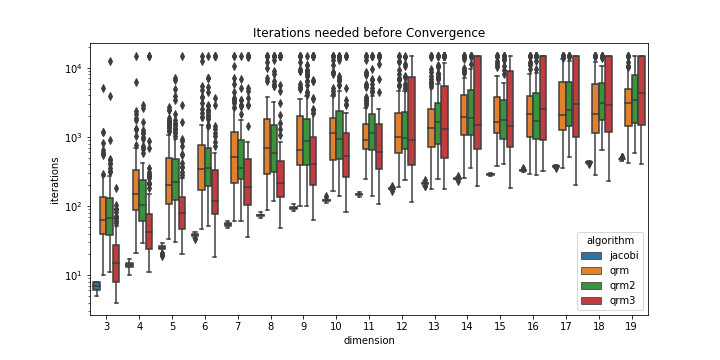
\includegraphics[width=11.5cm, height=5cm]{../media/plots/iterations_boxplot.png}

\end{center}
\end{figure}
}


%%%%%%%%%%%%%%%%%%%%%%%%%%%%%%%%%%%%%%%%%%%%%%%%%%%%%%%%%%%%%%%%%%%%%%%%%%%%%%%%%%%%%%%%%%%%%%%%%%%%%%%%
\frame[label=PCA-proof]{
\frametitle{PCA: proof}
The objective of \hyperlink{PCA-prop}{\beamergotobutton{PCA}}:
	$$
	max\ \delta^{\prime} Var \left(X\right) \delta \; s.t. \; \sum \delta_i^2 = 1
	$$
Corresponding Lagrangean:
    $$
    \mathcal{L}(Var \left(X\right), \delta, \lambda) =
    \delta^{\prime} Var \left(X\right) \delta - \lambda \left(\delta^{\prime}\delta - 1\right),
    $$
    where $\lambda \in \mathbb{R}^m$ \\
First order condition:
	\begin{align}
	\frac{\partial \mathcal{L}}{\partial \delta} &\stackrel{!}{=} 0 \notag\\
	2Var(X)\delta - 2\lambda_k \delta &\stackrel{!}{=} 0 \notag\\
	Var(X)\delta  &= \lambda_k \delta \notag
	\end{align}
Which is now reduced to a common Eigenvalue problem.
}
%%%%%%%%%%%%%%%%%%%%%%%%%%%%%%%%%%%%%%%%%%%%%%%%%%%%%%%%%%%%%%%%%%%%%%%%%%%%%%%%%%%%%%%%%%%%%%%%%%%%%%%%
\frame[label=LDA-proof]{
\frametitle{LDA: proof}
The objective of \hyperlink{LDA-prop}{\beamergotobutton{LDA}}:
  $$ max \ \frac{w^{\prime}S_B w}{w^{\prime}S_W w},$$
Which we can reformulate to:
  $$ max w^{\prime}S_B w \ s.t. w^{\prime}S_W w = 1. $$
Corresponding Lagrangean:
  $$ \mathcal{L}(w, S_B, S_W, \lambda) = w^{\prime}S_B w - \lambda \left(w^{\prime}S_W w - 1\right)$$
}
%%%%%%%%%%%%%%%%%%%%%%%%%%%%%%%%%%%%%%%%%%%%%%%%%%%%%%%%%%%%%%%%%%%%%%%%%%%%%%%%%%%%%%%%%%%%%%%%%%%%%%%%
\frame{
\frametitle{LDA: proof}
First order condition:
\begin{align*}
\frac{\partial \mathcal{L}}{\partial w} &\stackrel{!}{=} 0 \notag \\
2S_B w - 2 \lambda S_W w &\stackrel{!}{=} 0 \notag \\
S_{W}^{-1}S_B w &= \lambda w, \\
\end{align*}

which is known as a generalized Eigenvalue problem. We can redefine
\begin{align*}
S_B &= S_B^{\frac{1}{2}} S_B^{\frac{1}{2}} \\
v &= S_B^{\frac{1}{2}} w
\end{align*}
}
\frame{
\frametitle{LDA: proof}
We then get:
\begin{align*}
S_{W}^{-1}S_B w &= \lambda w \\
S_{W}^{-1}S_B^{\frac{1}{2}} \underbrace{S_B^{\frac{1}{2}} w}_v  &= \lambda w \\
S_B^{\frac{1}{2}} S_{W}^{-1}S_B^{\frac{1}{2}} v  &=\lambda \underbrace{S_B^{\frac{1}{2}} w}_v
\end{align*}
We can also rewrite this as:
$$S_B^{-\frac{1}{2}}S_{W}^{-1}S_B^{-\frac{1}{2}} v = \lambda v$$

Which now an Eigenvalue problem of a symmetric, positive semidefinite matrix \hyperlink{LDA-prop}{\beamergotobutton{back}}.

}
%%%%%%%%%%%%%%%%%%%%%%%%%%%%%%%%%%%%%%%%%%%%%%%%%%%%%%%%%%%%%%%%%%%%%%%%%%%%%%%%%%%%%%%%%%%%%%%%%%%%%%%%
\frame[label=similarity_proof]{
\frametitle{Eigenvalues of similar matrices}
From the definition in (\ref{similarity-prop}) it follows immediately that a matrix $A$ with Eigenvalues $\lambda_1, \dots, \lambda_n$ is similar to the matrix $diag(\lambda_1, \dots, \lambda_n)$.

If $A$ and $B$ are similar, as in (\ref{similarity-prop}), it holds:
\begin{align*}
B - \lambda I &= P^{-1} B P - \lambda P^{-1} I P \notag \\
              &= A - \lambda I.
\end{align*}
 Hence $A$ and $B$ have the same eigenvalues. Additionally, important transformations are based around orthogonal matrices. If $Q$ is orthogonal and
\begin{equation*}
A = Q^{\prime} B Q,
\end{equation*}
$A$ and $B$ are said to be \textit{orthogonally similar} \hyperlink{similarity_prop}{\beamergotobutton{back}}.
}
%%%%%%%%%%%%%%%%%%%%%%%%%%%%%%%%%%%%%%%%%%%%%%%%%%%%%%%%%%%%%%%%%%%%%%%%%%%%%%%%%%%%%%%%%%%%%%%%%%%%%%%%%
\frame[label=companion_exmpl]{
\frametitle{Companion-Matrix: Example}
Demonstrate that the companion matrix \hyperlink{companion_prop}{\beamergotobutton{back}}:
\begin{enumerate}
  \item corresponds to a polynomial.
  \item has eigenvalues equal to the roots of the polynomial.
\end{enumerate}
 $$A = \begin{bmatrix}
           0    & 1 \\
           -a_0 & -a_1 \\
       \end{bmatrix}$$

  \begin{align*}
      det \left(A - \lambda I\right) &= \begin{bmatrix}
                                            0 - \lambda    & 1 \\
                                            -a_0           & -a_1- \lambda \\
       \end{bmatrix} \\
                                     &= -\lambda\left(-a_1 - \lambda\right) + a_0 \\
                                     &= \lambda^2 + a_1 \lambda + a_0
  \end{align*}

}

%%%%%%%%%%%%%%%%%%%%%%%%%%%%%%%%%%%%%%%%%%%%%%%%%%%%%%%%%%%%%%%%%%%%%%%%%%%%%%%%%%%%%%%%%%%%%%%%%%%%%%%%%

\frame[label=householder_proof]{
\frametitle{Householder Reflections: proof}
\hyperlink{householder_prop}{\beamergotobutton{back}}
Remember:
\begin{itemize}
\item $Q = I - 2 uu^{\prime}$.
\item $u$ $v$ are orthonormal.
\end{itemize}

\begin{align*}
Qx &= c_1 u + c_2 v - 2c_1 uuu^{\prime} - 2 c_2 v uu^{\prime} \\
   &= c_1 u + c_2 v - 2c_1 u^{\prime}uu - 2 c_2 u^{\prime} v u \\
   &= -c_1 u + c_2 v\\
   &= \tilde{x}
\end{align*}
}

%%%%%%%%%%%%%%%%%%%%%%%%%%%%%%%%%%%%%%%%%%%%%%%%%%%%%%%%%%%%%%%%%%%%%%%%%%%%%%%%%%%%%%%%%%%%%%%%%%%%%%%%
\frame{
\frametitle{Sources}
\begin{thebibliography}{3}

\bibitem{NME}
Seffen B{\"o}rm and Christian Mehl.
Numerical Methods for Eigenvalue Problems.
Walter de Gruyter GmbH \& Co.KG, Berlin/Boston, 2012.

\bibitem{NLA}
James E. Gentle.
Numerical Linear Algebra for Applications in Statistics.
Springer Science + Business Media, New York, 2003.

\bibitem{MVA}
Wolfgang K. H{\"a}rdle and L{\'e}opold Simar.
Applied Multivariate Statistical Analysis.
Springer-Verlag Gmbh, Berlin, Heidelberg, 2015.

\end{thebibliography}
}

\end{document}

%%%%%%%%%%%%%%%%%%%%%%%%%%%%%%%%%%%%%%%%%%%%%%%%%%%%%%%%%%%%%%%%%%%%%%%%%%%%%%%%%%%%%%%%%%%%%%%%%%%%%%%%%
